\documentclass[titlepage,12pt,onehalfspacing]{article}
\usepackage{graphicx,setspace,natbib,fancyvrb,geometry,rotating}
\topmargin=-.2in\oddsidemargin=0pt\evensidemargin=0pt\textwidth=6.5in
\textheight=9in\headsep=.65in\headheight=0in

\begin{document}


\begin{singlespace}
\title{Determining Pump Pressure for a City Pipe Network}
\author{Cameron Bracken \\ENGR 325}
\date{\today}
\maketitle
\newpage
\pagenumbering{roman}\pagestyle{myheadings}
\tableofcontents\addcontentsline{toc}{section}{List of Figures}
\listoffigures \addcontentsline{toc}{section}{List of Tables}
\listoftables
\newpage
\end{singlespace}
\pagestyle{headings} \pagenumbering{arabic}
\section {Introduction}
A city pipe system is in need of a new pump.  The pipe system has a
minimum required pressure of 30 psi at each node (Figure 1).  A
minimum pump pressure must be determined to meet the minimum nodal
pressure requirements. In order to determine the minimum pump
pressure a linear relationship may be used as an approximation
(Finney 2006)

\begin{singlespacing}
\begin{equation}
a_{ij}=b_{ij}\left(p_i-p_j\right)
\end{equation}
where
\begin{center}
\begin{tabular}{rcl}
$a_{ij}$&=& Flowrate from node $i$ to node $j$ (Volume/time)\\
$b_{ij}$&=& Conductance factor for the pipe from node $i$ to node $j$ (Volume/time)\\
$p_i$&=& Pressure at at node (psi) $i$\\
\end{tabular}
\end{center}

\begin{figure}[h]
\begin{center}
\scalebox{1}{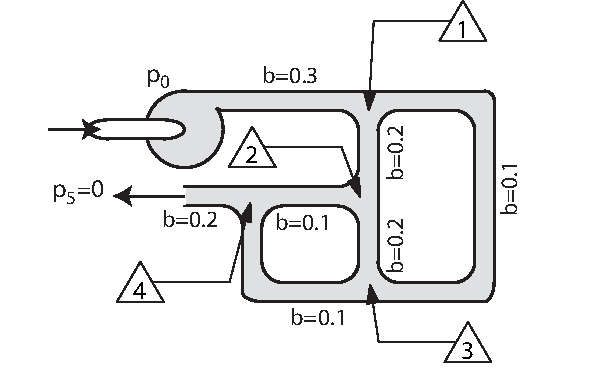
\includegraphics{figure1.pdf}} \caption{City pipe
network (Finney 2006)}
\end{center}
\end{figure}
\end{singlespacing}

\section{Methodology}
Equation 1 yields a system of four linear equations and four
unknowns (Finney 2006)
\begin{singlespacing}
\begin{center}
\begin{tabular}{rccccc}
Node 1:& $b_{01}(p_0-p_1)$ &=& $b_{12}(p_1-p_2)$ &+& $b_{13}(p_1-p_3)$\\
Node 2:& $b_{12}(p_1-p_2)$ &=& $b_{23}(p_2-p_3)$ &+& $b_{24}(p_2-p_4)$\\
Node 3:& $b_{13}(p_1-p_3)$ &+& $b_{23}(p_2-p_3)$ &=& $b_{34}(p_3-p_4)$\\
Node 3:& $b_{24}(p_2-p_4)$ &+& $b_{34}(p_3-p_4)$ &=& $b_{45}(p_4-p_5)$\\
\end{tabular}
\end{center}
\end{singlespacing}
The system can be simplified and written in matrix/vector form
$A$\underline{$x$}$=$\underline{$b$} for easy use.  Where A = the
coefficient matrix of conductance factors, \underline{$x$} = the
solution vector of pressure values and \underline{$b$} = the right
hand side vector of constant values.
\begin{displaymath}
\left[
\begin{array}{cccc}
(b_{01}+b_{12}+b_{13} & -b_{12} & -b_{13} & 0\\
-b_{13} & (b_{12}+b_{23}+b_{24}) & -b_{23} & -b_{24}\\
-b_{13} & -b_{23} & (b_{13}+b_{23}+b_{34}) & -b_{34}\\
0 & -b_{23} & -b_{34} & (b_{24}+b_{34}+b_{45})
\end{array}
\right]
\left[
\begin{array}{c}
p_1\\p_2\\p_3\\p_4
\end{array}
\right]
\begin{array}{c}
=
\end{array}
\left[
\begin{array}{c}
b_{01}p_0\\0\\0\\0\\
\end{array}
\right]
\end{displaymath}

To solve the system above, the technique of Gauss elimination can be
used. To utilize this technique the coefficient matrix A must first
be augmented with the right hand side vector \underline{$b$} to get
a new matrix [A$|$\underline{b}].   Gauss elimination is an
technique that is used to transform a matrix of the form
[A$|$\underline{b}] into an upper triangular form which can be
solved easily by back substitution.  The algorithm takes the form
\begin{displaymath}
row_{inew}=row_{iold}-\left(\frac{a_{i,j}}{a_{j,j}}\right)row_j
\end{displaymath}
Where $a_{k,k}$ = element of matrix [A$|$\underline{b}].  This
equation must be applied to every row of the working matrix.

Gauss elimination is an iterative procedure and is therefore ideal
for programming.  Program \verb pipe_network  (Appendix A) carries
out a version of the Gauss elimination process process called
forward elimination (Figure 2). The user may choose to scale and/or
pivot before the Gauss elimination starts.  A matrix singularity
tolerance must also be chosen to determine if the solution is
unique.  A non-singular matrix is one in which all if its rows and
columns are linearly independent.  A system involving a singular
matrix will have no unique solution.
\begin{figure}[!h]
\begin{center}
\begin{Verbatim}[frame=single]
  do j=1,neqn                        !this whole loop for gauss elimination
    if(pivot)then
      (carry out row interchange)
    end if
    if(abs(AB(j,j))<tol)then              !user specified tolerance
      (NO SOLUTION),stop
    end if
    do i=j+1,neqn
      hold=AB(i,j)/AB(j,j)
      do k=j,neqn+nrhs
        AB(i,k)=AB(i,k)-(hold)*AB(j,k)   !row reduction
      end do
    end do
  end do
\end{Verbatim}
\caption{Gauss elimination algorithm}
\end{center}
\end{figure}

The determinate of a matrix is an indicator of how
singular that matrix is. Once program \verb pipe_network  has
created an upper triangular matrix from [A$|$\underline{b}] then the
determinate can be calculated by multiplying the diagonal elements
of matrix A
\begin{displaymath}
det(A)=\left(\prod_{i=1}^{neqn}a_{ii}\right)det
\end{displaymath}
where det = the product of the scale factors $\times$
$(-1)^{\#pivots}$ and $neqn$ = \# of equations. \pagebreak

Calculations involving numbers with either large or small magnitudes
can introduce roundoff error.  To reduce roundoff error, the
technique of scaling can be used (Figure 3).  To scale a matrix,
divide each row by the entry in that row with the largest absolute
magnitude. All values in the resulting matrix will be $<$1.
\begin{figure}[!h]
\begin{center}
\begin{Verbatim}[frame=single]
  det=1d0                    !to scale
  if(scale)then
    do i=1,neqn
      max=0d0
      do j=1,neqn+nrhs
        if(abs(A(i,j))>abs(max))then
          max=A(i,j)
        end if
      end do
      AB(i,1:neqn+nrhs)=AB(i,1:neqn+nrhs)/max
      det=det*max
    end do
  end if
\end{Verbatim}
\caption{Scaling}
\end{center}
\end{figure}

Pivoting (row interchange)is another technique used to reduce
roundoff error (Figure 4). Pivoting attempts to minimize the value
of $\frac{a_{i,j}}{a_{j,j}}row_j$ from equation 1.  To minimize
$\frac{a_{i,j}}{a_{j,j}}row_j$, $a_{j,j}$ must be large and
therefore the process of pivoting also reduces the chance of
division by zero.

\begin{figure}[!h]
\begin{center}
\begin{Verbatim}[frame=single]
  if(pivot)then
    do i=j,neqn                    !check for row max
      if(abs(AB(i,j))>abs(AB(imax,j)))then
        imax=i
      end if
    end do
    if(imax/=j)then
      do k=j,neqn+nrhs
        hold=AB(j,k)
        AB(j,k)=AB(imax,k)        !row interchange
        AB(imax,k)=hold
      end do
  end if
\end{Verbatim}
\caption{Pivoting (row interchange)}
\end{center}
\end{figure}

After the matrix [A$|$\underline{b}] has been triangularized, back
substitution can be used to solve for the pressure values.  Back
substitution starts with the last row and works up the matrix,
successively solving for the pressure values (Figure 5).

\begin{figure}[!h]
\begin{center}
\begin{Verbatim}[frame=single]
  do k=1,nrhs                    !back substitution, last row first
    x(neqn,k)=AB(neqn,neqn+k)/AB(neqn,neqn)
    do i=neqn-1,1,-1             !rest of rows working up
      sum=0
      do j=i+1,neqn
        sum=sum+x(j,k)*AB(i,j)
      end do
      x(i,k)=(AB(i,neqn+k)-sum)/AB(i,i)
    end do
  end do
\end{Verbatim}
\caption{Back substitution}
\end{center}
\end{figure}
\section{Application}
The pressure at each node is dependent on the conductance factor
($b_{ij}$) and the pump pressure (psi) (Table 1).
\begin{table}[h]
\begin{center}
\caption{Parameters associated with determining nodal pressure}
% Table generated by Excel2LaTeX from sheet 'Sheet3'
\begin{tabular}[!h]{|r|r|r|}
\hline
{\bf Parameter} & {\bf Variable} & {\bf Value} \\
\hline
Pump Pressure & $p_0$ & 80psi \\
\hline
Conductance factor from & $b_{01}$ &   0.3 \\

node 0 to node 1 &       &       \\
\hline
      & $b_{12}$ &   0.2 \\
\hline
      & $b_{13}$ &   0.1 \\
\hline
      & $b_{23}$ &   0.2 \\
\hline
      & $b_{24}$ &   0.1 \\
\hline
      & $b_{34}$ &   0.1 \\
\hline
      & $b_{45}$ &   0.2 \\
\hline
\end{tabular}
\end{center}
\end{table}

To test the sensitivity of the system, different parameters can be
varied (Table 2).

\begin{table}[h]
\begin{center}
\caption{Variation of Parameters}
% Table generated by Excel2LaTeX from sheet 'Sheet3'
\begin{tabular}{|c|r|r|r|r|}
\hline
{\bf Run \#} & {\bf Variable} & {\bf Initial value} & {\bf New value} & {\bf Variation} \\
\hline
         1 &     $p_0$ &     80 psi &       88.0 &       10\% \\

 \hline
         3 &  $b_{01}$ &        0.3 &       0.33 &       10\% \\

 \hline
         5 &  $b_{12}$ &        0.2 &       0.22 &       10\% \\

\hline
         7 &  $b_{13}$ &        0.1 &       0.11 &       10\% \\

 \hline
         9 &  $b_{23}$ &        0.2 &       0.22 &       10\% \\

\hline
        11 &  $b_{24}$ &        0.1 &       0.11 &       10\% \\

\hline
        13 &  $b_{34}$ &        0.1 &       0.11 &       10\% \\

 \hline
        15 &  $b_{45}$ &        0.2 &       0.22 &       10\% \\

 \hline
\end{tabular}
\end{center}
\end{table}

\section{Results}
Inputting the values from Table 1 into the initial system of
equations results in the solvable linear system
\begin{displaymath}
\left[
\begin{array}{cccc}
.6 & -.2 & -.1 & 0\\
-.1 & .5 & -.2 & -.1\\
-.1 & -.2 & .4 & -.1\\
0 & -.1 & -.1 & .4
\end{array}
\right] \left[
\begin{array}{c}
p_1\\p_2\\p_3\\p_4
\end{array}
\right]
\begin{array}{c}
=
\end{array}
\left[
\begin{array}{c}
24\\0\\0\\0\\
\end{array}
\right]
\end{displaymath}
\verb pipe_network  can be use to find that the solution vector
\begin{displaymath}
p =\left[
\begin{array}{cccc}
64.084 & 49.005 & 46.492 & 23.874
\end{array}
\right]^T
\end{displaymath}

The pressure value at $p_4$ is well under the minimum pressure of 30
psi.  Increasing the pump pressure accordingly reveals that a 103.6
psi pump would give a pressure at node 4 of just over 30 psi (Table
3). The pump would most likely have to be a more standard size of
110 psi.
\begin{table}[h]
\begin{center}
\caption{Determining minimum pump pressure}
% Table generated by Excel2LaTeX from sheet 'Sheet3'
\begin{tabular}{|l|l|}
\hline
{\bf Pump Pressure} & {\bf Node 4 Pressure } \\
\hline
    80 psi & 23.874 psi \\
\hline
    90 psi & 26.859 psi \\
\hline
   100 psi & 29.843 psi \\
\hline
100.16 psi & 30.022 psi \\
\hline
   110 psi & 32.827 psi \\
\hline
\end{tabular}
\end{center}
\end{table}

The sensitivity analysis reveals how the nodal pressure changes with
the variation of parameters (negative variation values are opposite
but show a similar trend so are therefore excluded).  The largest
change in nodal pressure values is seen when pump pressure ($p_0$)
is increased.  The smallest change is seen when $b_{23}$ is varied.
\begin{table}[h]
\caption{Sensitivity analysis}
% Table generated by Excel2LaTeX from sheet 'Sheet2'
\begin{tabular}{|c|r|c|r|c|c|c|c|c|c|c|c|} \hline
{\begin{sideways}\bf Run \#\end{sideways}} & {\begin{sideways}\bf Variable\end{sideways}} & {\begin{sideways}\bf New Value\end{sideways}} & {\begin{sideways}\bf Variation\end{sideways}} & {\bf $p_1$} & {\bf $p_2$} & {\bf $p_3$} & {\bf $p_4$} & {\bf $\Delta p_1$} & {\bf $\Delta p_2$} & {\bf $\Delta p_3$} & {\bf $\Delta p_4$} \\
\hline
    1 & $p_0$ &  88.0 &  10\% & 70.490 & 53.906 & 51.141 & 26.262 & 9.09\% & 9.09\% & 9.09\% & 9.09\% \\
\hline
    2 & $b_{01}$ &  0.33 &  10\% & 65.264 & 49.908 & 47.349 & 24.314 & 1.81\% & 1.81\% & 1.81\% & 1.81\% \\
\hline
    3 & $b_{12}$ &  0.22 &  10\% & 63.905 & 49.704 & 46.864 & 24.142 & -0.28\% & 1.41\% & 0.79\% & 1.11\% \\
\hline
    4 & $b_{13}$ &  0.11 &  10\% & 63.960 & 49.209 & 47.033 & 24.060 & -0.19\% & 0.41\% & 1.15\% & 0.77\% \\
\hline
    5 & $b_{23}$ &  0.22 &  10\% & 64.079 & 48.946 & 46.581 & 23.882 & -0.01\% & -0.12\% & 0.19\% & 0.03\% \\
\hline
    6 & $b_{24}$ &  0.11 &  10\% & 63.831 & 48.386 & 46.214 & 24.253 & -0.40\% & -1.28\% & -0.60\% & 1.56\% \\
\hline
    7 & $b_{34}$ &  0.11 &  10\% & 63.880 & 48.722 & 45.835 & 24.180 & -0.32\% & -0.58\% & -1.43\% & 1.27\% \\
\hline
    8 & $b_{45}$ &  0.22 &  10\% & 64.640 & 48.141 & 45.558 & 22.309 & 0.86\% & -1.79\% & -2.05\% & -7.02\% \\
\hline
\end{tabular}
\end{table}

A stacked graph of the variation shows the percent change in
pressure in relation to each conductance factor increase (Figure 6).
Increasing the conductance factors near the pump will increase nodal
pressure but increasing the conductance factors near the system
output will decrease nodal pressure.

\begin{figure}[!h]
\begin{center}
\scalebox{.75}{\includegraphics{increase.jpg}} \\
\caption{Total change in pressure due to increase of individual
conductance factors.}
\end{center}
\end{figure}

\section{Conclusion}
The following can be concluded from this model:
\begin{itemize}
\item{The pressure values that an 80 psi pump will yield are 64.084, 49.005, 46.492, and 23.874 psi respectively.}
\item{Pump pressure is the most influential parameter.}
\item{A 110 psi pump will satisfy the minimum pressure requirement
of 30 psi at all nodes.}
\item{An increase in the conductance factors near the pump will
increase nodal pressure.}
\item{An increase in conductance factors near the system output will
decrease nodal pressure.}
\end{itemize}

\section{References}
Finney, Brad. Lab 8 handout, Humboldt State University, Spring 2006.

\appendix
\newcommand{\appsection}[1]{\let\oldthesection\thesection
  \renewcommand{\thesection}{Appendix \oldthesection}
  \section{#1}\let\thesection\oldthesection}
\appsection{\\~Source Code and Program Output} \label{sec:source}
\begin{singlespacing}
\begin{Verbatim}[frame=single]
Script started on Mon 10 Apr 2006 02:01:30 PM DT
cwb12@ere-server:~/engr325/lab8> cat lab8.3.f90

program pipe_network
  implicit none
  double precision,allocatable,dimension(:,:)::A,b,x
  double precision,allocatable,dimension(:,:)::rowef
  double precision::det,b01,b12,b13,b23,b24,b34,b45,p0,tol
  integer::neqn,nrhs,i,j,check
  character(len=1)::ans
  character(len=30)::file
  logical::scale,solution,pivot

  interface
    subroutine gauss(A,b,x,ref,neqn,nrhs,scale,solution,det,pivot,tol)
      double precision,dimension(:,:),intent(in)::A,b
      double precision,dimension(:,:),intent(out)::x
      double precision,dimension(neqn,neqn+nrhs),intent(out)::ref
      double precision,intent(in)::tol
      double precision,intent(out)::det
      integer,intent(in)::neqn,nrhs
      logical,intent(in)::scale,pivot
      logical,intent(out)::solution
    end subroutine gauss
  end interface

  !This Program will read in a square coefficient matrix A and a right
  !hand side vector b and call a gauss elimination subroutine to find
  !the solution vector x.
  !~~It can handle b and x vector with rank>1~~
  !variable list:
  !--inputs:
  !A       =coefficient matrix(pressure values in this case)
  !         must be square
  !b       =right hand side vector
  !neqn    =number of equations/unknowns in matrix A (number of rows)
  !nrhs    =number of columns in right hand side vector b
  !ans     =answer to "do you want to scale"
  !file    =name of file containing data
  !pivot   =if ans is yes then pivot=.true. else pivot=.false.
  !tol     =singularity tolerance for diagonal elements
  !--outputs:
  !x       =solution vector
  !det     =determinant of matrix A
  !ref     =row eschelon form of marrix A|b
  !--internal variables:
  !i,j     =loop variables
  !check   =iostat check for read ans
  !scale   =if ans is yes then scale=.true. else scale=.false.
  !solution=if the system has a solution then solution=.true.

  write(*,*)"This program will read in a square coefficient matrix A"
  write(*,*)"of pressure values and a right hand side vector b and call a"
  write(*,*)"gauss elimination subroutine to find the solution vector x."
  write(*,*)" "
  write(*,*)"Enter the name of the file that contains the initial pressure"
  write(*,*)"and friction coefficients of matrix A and vector b."
  read(*,"(a)")file
  open(11,file=file)
  neqn=4
  nrhs=1
  allocate(A(neqn,neqn),b(neqn,nrhs),x(neqn,nrhs),rowef(neqn,neqn+nrhs))
  do
    read(11,*,iostat=check)p0,b01,b12,b13,b23,b24,b34,b45
    if(check/=0)then
      write(*,*)"something is wrong, check your file and try again."
      exit
      stop
    else if(check==0)then
      exit
    end if
  end do

  A(1,1)=(b01+b12+b13)
  A(1,2)=-b12
  A(1,3)=-b13
  A(1,4)=0
  A(2,1)=-b12
  A(2,2)=(b12+b23+b24)
  A(2,3)=-b23
  A(2,4)=-b24
  A(3,1)=-b13
  A(3,2)=-b23
  A(3,3)=(b13+b23+b34)
  A(3,4)=-b34
  A(4,1)=0
  A(4,2)=-b24
  A(4,3)=-b34
  A(4,4)=(b24+b34+b45)
  b(1,1)=b01*p0
  b(2,1)=0
  b(3,1)=0
  b(4,1)=0

  write(*,*)"Enter the matrix singularity tolerance"
  read(*,*)tol
  do
    write(*,*)"Do you want to scale matrix A|B? (y or n)"
    read(*,"(a)",iostat=check)ans
    if(ans=="y" .and. check==0)then
      scale=.true.
      exit
    else if(ans=="n")then
      scale=.false.
      exit
    else if(check/=0)then
      write(*,*)"Not an option."
    end if
  end do
  do
    write(*,*)"Do you want to use pivoting? (y or n)"
    read(*,"(a)",iostat=check)ans
    if(ans=="y" .and. check==0)then
      pivot=.true.
      exit
    else if(ans=="n")then
      pivot=.false.
      exit
    else if(check/=0)then
      write(*,*)"Not an option."
    end if
  end do

  call gauss(A,b,x,rowef,neqn,nrhs,scale,solution,det,pivot,tol)

  if(solution)then
    write(*,*)"ref(A|b)="
    do i=1,neqn
      write(*,"(a)",advance="no")"|"
      write(*,"(100f8.3)",advance="no")(rowef(i,j),j=1,nrhs+neqn)
      write(*,"(a)")"|"
    end do
    write(*,*)" "
    write(*,*)"The solution vector:"
    write(*,*)"x="
    do i=1,neqn
      write(*,"(100f10.3)")(x(i,j),j=1,nrhs)
    end do
    write(*,"(/,a8,f8.5,/)")" det(A)=",det
  end if
  stop
end program pipe_network


subroutine gauss(A,b,x,ref,neqn,nrhs,scale,solution,det,pivot,tol)
  implicit none
  double precision,dimension(:,:),intent(in)::A,b
  double precision,dimension(:,:),intent(out)::x
  double precision,dimension(neqn,neqn+nrhs),intent(out)::ref
  double precision,intent(out)::det
  double precision,intent(in)::tol
  integer,intent(in)::neqn,nrhs
  logical,intent(in)::scale,pivot
  logical,intent(out)::solution
  double precision,dimension(neqn,neqn+nrhs)::AB
  double precision,dimension(neqn+nrhs)::dummy
  double precision::max,sum,hold
  integer::maxpos,row,i,j,k,l,imax

  !This subroutine will input an coefficient matrix A and a right hand
  !side matrix b from the form Ax=b, augment one with the other to get
  !a new matrix AB, scale if desired, find the ref of the AB, and using
  !back substitution, find the solution matrix x associated with A and b.
  !~~b may be a vector or a matrix~~
  !variable list:
  !--inputs:
  !A        =coefficient matrix(pressure values in this case)
  !          must be square
  !b        =right hand side vector
  !neqn     =number of equations/unknowns in matrix A (number of rows)
  !nrhs     =number of columns in right hand side vector b
  !scale    =if ans is yes then scale=.true. else scale=.false.
  !pivot    =if ans is yes then pivot=.true. else pivot=.false.
  !tol      =matrix singularity tolerance
  !--outputs:
  !x        =solution vector
  !det      =determinant of matrix A
  !ref      =row eschelon form of matrix A|b
  !solution =if the system has a solution then solution=.true.
  !--internal variables:
  !AB       =matrix A augmented with matrix b
  !max      =max of row, used for scaling
  !row      =working row for augmentation
  !sum      =sum of terms used in back substitution
  !hold     =temporary hold of values in row reduction and row interchange
  !imax     =row with max value for each working column (used to indicate if
  !          row interchange is necessary
  !i,j,k,l  =loop variables


  AB=A
  row=0
  do j=neqn+1,neqn+nrhs    !Augment A with b
    row=row+1
    do i=1,neqn
      AB(i,j)=b(i,row)
    end do
  end do

  det=1d0
  if(scale)then       !This if,then statement is to scale
    do i=1,neqn
      max=0d0
      maxpos=1
      do j=1,neqn+nrhs
        if(abs(A(i,j))>abs(max))then
          max=A(i,j)
          maxpos=j
        end if
      end do
      AB(i,1:neqn+nrhs)=AB(i,1:neqn+nrhs)/max
      det=det*max
    end do
  end if


  do j=1,neqn                        !this whole loop for gauss ref
    imax=1
    if(pivot)then
      do i=j,neqn                    !check for row max
        if(abs(AB(i,j))>abs(AB(imax,j)))then
          imax=i
        end if
      end do
      if(imax/=j)then
        do k=j,neqn+nrhs
          hold=AB(j,k)
          AB(j,k)=AB(imax,k)        !row interchange
          AB(imax,k)=hold
               !write(*,*)"  ",k
          end do
        end if
    end if
    solution=.true.
    if(abs(AB(j,j))<tol)then
      solution=.false.
      write(*,*)"NO SOLUTION"
      return
      stop
    end if
    do i=j+1,neqn                    !row reduction
      hold=AB(i,j)/AB(j,j)
      do k=j,neqn+nrhs
        AB(i,k)=AB(i,k)-(hold)*AB(j,k)
      end do
    end do
  end do

  do k=1,nrhs                    !back substitution, last row first
    x(neqn,k)=AB(neqn,neqn+k)/AB(neqn,neqn)
    do i=neqn-1,1,-1             !rest of rows working up
      sum=0
          !sum(AB(i,i+1:neqn)*x(i+1:neqn,k))
      do j=i+1,neqn
        sum=sum+x(j,k)*AB(i,j)
      end do
      x(i,k)=(AB(i,neqn+k)-sum)/AB(i,i)
    end do
  end do

  do i=1,neqn
    det=det*AB(i,i)        !calculate the determinate by multiplying
  end do                   !diagonal elements because AB is triangular

  ref=0
  do i=1,neqn              !divide each row by leading entry to get ref
    ref(i,1:neqn+nrhs)=AB(i,1:neqn+nrhs)/AB(i,i)
  end do

  return
end subroutine gauss

cwb12@ere-server:~/engr325/lab8> ifort lab8.3.f90
cwb12@ere-server:~/engr325/lab8> lab8
 This program will read in a square coefficient matrix A
 of pressure values and a right hand side vector b and call a
 gauss elimination subroutine to find the solution vector x.

 Enter the name of the file that contains the initial pressure
 and friction coefficients of matrix A and vector b.
bval.dat
 Enter the matrix singularity tolerance
.000001
 Do you want to scale matrix A|B? (y or n)
n
 Do you want to use pivoting? (y or n)
y
 ref(A|b)=
|   1.000  -0.333  -0.167   0.000  40.000|
|   0.000   1.000  -0.538  -0.231  18.462|
|   0.000   0.000   1.000  -0.597  32.239|
|   0.000   0.000   0.000   1.000  23.874|

 The solution vector:
 x=
    64.084
    49.005
    46.492
    23.874

 det(A)= 0.01910

cwb12@ere-server:~/engr325/lab8> cat bval.dat\\
 80 .3 .2 .1 .2 .1 .1 .2
cwb12@ere-server:~/engr325/lab8> exit exit Script done on Mon 10 Apr
2006 02:02:55 PM PDT
\end{Verbatim}
\end{singlespacing}
\noindent This was typeset with \LaTeX
\end{document}
